\part{Introduction}

Computer science (abbreviated CS or CompSci) is the scientific and practical approach to computation and its applications. It is the systematic study of the feasibility, structure, expression, and mechanization of the methodical processes (or algorithms) that underlie the acquisition, representation, processing, storage, communication of, and access to information, whether such information is encoded in bits and bytes in a computer memory or transcribed engines and protein structures in a human cell. A computer scientist specializes in the theory of computation and the design of computational systems.

Its subfields can be divided into a variety of theoretical and practical disciplines. Some fields, such as computational complexity theory (which explores the fundamental properties of computational problems), are highly abstract, while fields such as computer graphics emphasize real-world visual applications. Still other fields focus on the challenges in implementing computation. For example, programming language theory considers various approaches to the description of computation, whilst the study of computer programming itself investigates various aspects of the use of programming language and complex systems. Human-computer interaction considers the challenges in making computers and computations useful, usable, and universally accessible to humans.

计算机科学(Computer Science,有时缩写为CS)是系统性研究信息与计算的理论基础以及它们在计算机系统中如何实现与应用的实用技术的学科。它通常被形容为对那些创造、描述以及转换信息的算法处理的系统研究。计算机科学包含很多分支领域;其中一些,比如计算机图形学强调特定结果的计算,而另外一些,比如计算复杂性理论是学习计算问题的性质。还有一些领域专注于挑战怎样实现计算。比如程序设计语言理论学习描述计算的方法,而程序设计是应用特定的程序设计语言解决特定的计算问题,人机交互则是专注于挑战怎样使计算机和计算变得有用、可用,以及随时随地为人所用。

有时公众会误以为计算机科学就是解决计算机问题的事业(比如信息技术),或者只是与使用计算机的经验有关,如玩游戏、上网或者文字处理。其实计算机科学所关注的,不仅仅是去理解实现类似游戏、浏览器这些软件的程序的性质,更要通过现有的知识创造新的程序或者改进已有的程序。

\chapter{History}

The earliest foundations of what would become computer science predate the invention of the modern digital computer. Machines for calculating fixed numerical tasks such as the abacus have existed since antiquity but they only supported the human mind, aiding in computations as complex as multiplication and division.

Blaise Pascal designed and constructed the first working mechanical calculator, Pascal's calculator, in 1642. Two hundred years later, Thomas de Colmar launched the mechanical calculator industry when he released his simplified arithmometer, which was the first calculating machine strong enough and reliable enough to be used daily in an office environment. Charles Babbage started the design of the first automatic mechanical calculator, his difference engine, in 1822, which eventually gave him the idea of the first programmable mechanical calculator, his Analytical Engine. He started developing this machine in 1834 and "in less than two years he had sketched out many of the salient features of the modern computer. A crucial step was the adoption of a punched card system derived from the Jacquard loom"[6] making it infinitely programmable. In 1843, during the translation of a French article on the analytical engine, Ada Lovelace wrote, in one of the many notes she included, an algorithm to compute the Bernoulli numbers, which is considered to be the first computer program. Around 1885, Herman Hollerith invented the tabulator which used punched cards to process statistical information; eventually his company became part of IBM. In 1937, one hundred years after Babbage's impossible dream, Howard Aiken convinced IBM, which was making all kinds of punched card equipment and was also in the calculator business[9] to develop his giant programmable calculator, the ASCC/Harvard Mark I, based on Babbage's analytical engine, which itself used cards and a central computing unit. When the machine was finished, some hailed it as "Babbage's dream come true".

During the 1940s, as new and more powerful computing machines were developed, the term computer came to refer to the machines rather than their human predecessors. As it became clear that computers could be used for more than just mathematical calculations, the field of computer science broadened to study computation in general. Computer science began to be established as a distinct academic discipline in the 1950s and early 1960s. The world's first computer science degree program, the Cambridge Diploma in Computer Science, began at the University of Cambridge Computer Laboratory in 1953. The first computer science degree program in the United States was formed at Purdue University in 1962. Since practical computers became available, many applications of computing have become distinct areas of study in their own right.

Although many initially believed it was impossible that computers themselves could actually be a scientific field of study, in the late fifties it gradually became accepted among the greater academic population. It is the now well-known IBM brand that formed part of the computer science revolution during this time. IBM (short for International Business Machines) released the IBM 704 and later the IBM 709 computers, which were widely used during the exploration period of such devices. "Still, working with the IBM [computer] was frustrating...if you had misplaced as much as one letter in one instruction, the program would crash, and you would have to start the whole process over again". During the late 1950s, the computer science discipline was very much in its developmental stages, and such issues were commonplace.

Time has seen significant improvements in the usability and effectiveness of computing technology. Modern society has seen a significant shift in the users of computer technology, from usage only by experts and professionals, to a near-ubiquitous user base. Initially, computers were quite costly, and some degree of human aid was needed for efficient use - in part from professional computer operators. As computer adoption became more widespread and affordable, less human assistance was needed for common usage.

早期计算机科学创建的基础得追溯到现代电子计算机的发明。那些计算固定数值任务的机器,比如算盘,自古希腊时期即已存在。Wilhelm Schickard在1623年设计了世界上第一台机械计算器,但没有完成它的建造。布莱兹·帕斯卡在1642年设计并且建造了世界上第一台可以工作的机械计算器Pascaline。埃达·洛夫莱斯协助查尔斯·巴贝奇在维多利亚时代设计了差分机。1900年左右,打孔机问世。然而以上这些机器都局限在只能完成单个任务,或者充其量是所有可能任务的子集。


到了20世纪40年代,随着更新更强大的计算机器被发明,术语“计算机”开始用于指代那些机器而不是它们的祖先。计算机的概念变得更加清晰,它不仅仅用于数学运算,总的来说计算机科学的领域也扩展到了对于计算的研究。20世纪50年代至20世纪60年代早期,计算机科学开始被确立为不同种类的学术学科。世界上第一个计算机科学学位点由普渡大学在1962年设立。随着实用计算机的出现,很多计算的应用都以它们自己的方式逐渐转变成了研究的不同领域。

虽然最初很多人并不相信计算机可能成为科学研究的领域,但是随后的50年里也逐渐被学术界认可。IBM公司是那段时期计算机科学革命的参与者之一。在那段探索时期,IBM(International Business Machines的缩写)发布的IBM 704以及之后的IBM 709计算机被广泛使用。“不过,使用IBM电脑工作仍然是一件很沮丧的事情。如果你弄错了一条指令中的一个字母,程序将会崩溃,而你也得从头再来。”到了20世纪60年代后期,计算机科学学科得到了长足发展,这在当时是一件很寻常的事情。


随着时间的推移,计算机科学技术在可用性和有效性上都有显著提升。现代社会见证了计算机从仅仅由专业人士使用到被广大用户接受的重大转变。最初,计算机非常昂贵,要有效利用它们,某种程度上必须得由专业的计算机操作员来完成。然而,随着计算机变得普及和低廉,已经几乎不需要专人的协助,虽然某些时候援助依旧存在。

\section{Major archievements}

Despite its short history as a formal academic discipline, computer science has made a number of fundamental contributions to science and society - in fact, along with electronics, it is a founding science of the current epoch of human history called the Information Age and a driver of the Information Revolution, seen as the third major leap in human technological progress after the Industrial Revolution (1750-1850 CE) and the Agricultural Revolution (8000-5000 BCE).

These contributions include:


\begin{compactitem}
\item The start of the "digital revolution," which includes the current Information Age and the Internet.

\item A formal definition of computation and computability, and proof that there are computationally unsolvable and intractable problems.

\item The concept of a programming language, a tool for the precise expression of methodological information at various levels of abstraction.

\item In cryptography, breaking the Enigma code was an important factor contributing to the Allied victory in World War II.

\item Scientific computing enabled practical evaluation of processes and situations of great complexity, as well as experimentation entirely by software. It also enabled advanced study of the mind, and mapping of the human genome became possible with the Human Genome Project. Distributed computing projects such as Folding@home explore protein folding.

\item Algorithmic trading has increased the efficiency and liquidity of financial markets by using artificial intelligence, machine learning, and other statistical and numerical techniques on a large scale. High frequency algorithmic trading can also exacerbate volatility.

\item Computer graphics and computer-generated imagery have become almost ubiquitous in modern entertainment, particularly in television, cinema, advertising, animation and video games. Even films that feature no explicit CGI are usually "filmed" now on digital cameras, or edited or postprocessed using a digital video editor.

\item Simulation of various processes, including computational fluid dynamics, physical, electrical, and electronic systems and circuits, as well as societies and social situations (notably war games) along with their habitats, among many others. Modern computers enable optimization of such designs as complete aircraft. Notable in electrical and electronic circuit design are SPICE, as well as software for physical realization of new (or modified) designs. The latter includes essential design software for integrated circuits.

\item Artificial intelligence is becoming increasingly important as it gets more efficient and complex. There are many applications of the AI, some of which can be seen at home, such as robotic vacuum cleaners. It is also present in video games and on the modern battlefield in drones, anti-missile systems, and squad support robots.
\end{compactitem}



虽然计算机科学被认定为正式学术学科的历史很短暂,但仍对科学和社会作出了很多基础贡献。包括:


\begin{compactitem}
\item “数字革命”的开端:信息时代与互联网。

\item 对于计算和可计算理论的正式定义,证明了存在计算上不可解及难解型问题。

\item 程序设计语言的概念,一种在不同抽象级别上精确表达方法信息(methodological information)的工具。

\item 在密码学领域,恩尼格玛密码机的破译被视为盟军在二战取得胜利的重要因素。

\item 科学计算实现了高复杂度处理的实用价值,以及完全使用软件进行实验。同时也实现了对人类思想的深入研究,使得人类基因组计划绘制人类基因成为可能。还有探索蛋白质折叠的分布式计算项目Folding@home。

\item 算法交易增长了金融市场的经济效益与市场流通性,通过人工智能,机器学习及大规模的统计和数值技术。

\item 图像合成。

\item 自然语言处理,包括语音到文字(speech-to-text)转换、语言间的自动翻译[来源请求]
\item 对各种过程的模拟,包括计算流体力学、物理、电气、电子系统和电路,以及同人类居住地联系在一起的社会和社会形态(尤其是战争游戏,war games)。现代计算机能够对这些设计进行优化,如飞机设计。尤其在电气与电子电路设计中,SPICE软件对新的物理实现(或修改)设计具有很大帮助。它包含了针对集成电路的基本设计软件。
\end{compactitem}


\chapter{Philosophy}

A number of computer scientists have argued for the distinction of three separate paradigms in computer science. Peter Wegner argued that those paradigms are science, technology, and mathematics. Peter Denning's working group argued that they are theory, abstraction (modeling), and design. Amnon H. Eden described them as the "rationalist paradigm" (which treats computer science as a branch of mathematics, which is prevalent in theoretical computer science, and mainly employs deductive reasoning), the "technocratic paradigm" (which might be found in engineering approaches, most prominently in software engineering), and the "scientific paradigm" (which approaches computer-related artifacts from the empirical perspective of natural sciences, identifiable in some branches of artificial intelligence).

Peter Wegner和Amnon H. Eden提议了三种范式应用于计算机科学的各个领域:

\begin{compactitem}
\item “理性主义范式”,将计算机科学看作是数学的分支,在理论计算机科学中很流行,主要利用演绎推理。
\item “技术专家范式”,这类范式有着很明显的工程学倾向,尤其是在软件工程领域。
\item “科学范式”,人工智能的某些分支可以作为这类范式的代表(比如说对于人工生命的研究)。
\end{compactitem}




\section{Name of the field}

The term "computer science" appears in a 1959 article in Communications of the ACM,[27] in which Louis Fein argues for the creation of a Graduate School in Computer Sciences analogous to the creation of Harvard Business School in 1921, justifying the name by arguing that, like management science, the subject is applied and interdisciplinary in nature, while having the characteristics typical of an academic discipline. His efforts, and those of others such as numerical analyst George Forsythe, were rewarded: universities went on to create such programs, starting with Purdue in 1962. Despite its name, a significant amount of computer science does not involve the study of computers themselves. Because of this, several alternative names have been proposed. Certain departments of major universities prefer the term computing science, to emphasize precisely that difference. Danish scientist Peter Naur suggested the term datalogy, to reflect the fact that the scientific discipline revolves around data and data treatment, while not necessarily involving computers. The first scientific institution to use the term was the Department of Datalogy at the University of Copenhagen, founded in 1969, with Peter Naur being the first professor in datalogy. The term is used mainly in the Scandinavian countries. Also, in the early days of computing, a number of terms for the practitioners of the field of computing were suggested in the Communications of the ACM – turingineer, turologist, flow-charts-man, applied meta-mathematician, and applied epistemologist. Three months later in the same journal, comptologist was suggested, followed next year by hypologist.[34] The term computics has also been suggested. In Europe, terms derived from contracted translations of the expression "automatic information" (e.g. "informazione automatica" in Italian) or "information and mathematics" are often used, e.g. informatique (French), Informatik (German), informatica (Italy), informática (Spain, Portugal), informatika (Slavic languages) or pliroforiki (πληροφορική, which means informatics) in Greek. Similar words have also been adopted in the UK (as in the School of Informatics of the University of Edinburgh).

A folkloric quotation, often attributed to—but almost certainly not first formulated by—Edsger Dijkstra, states that "computer science is no more about computers than astronomy is about telescopes." The design and deployment of computers and computer systems is generally considered the province of disciplines other than computer science. For example, the study of computer hardware is usually considered part of computer engineering, while the study of commercial computer systems and their deployment is often called information technology or information systems. However, there has been much cross-fertilization of ideas between the various computer-related disciplines. Computer science research also often intersects other disciplines, such as philosophy, cognitive science, linguistics, mathematics, physics, statistics, and logic.


Computer science is considered by some to have a much closer relationship with mathematics than many scientific disciplines, with some observers saying that computing is a mathematical science. Early computer science was strongly influenced by the work of mathematicians such as Kurt Gödel and Alan Turing, and there continues to be a useful interchange of ideas between the two fields in areas such as mathematical logic, category theory, domain theory, and algebra.

The relationship between computer science and software engineering is a contentious issue, which is further muddied by disputes over what the term "software engineering" means, and how computer science is defined. David Parnas, taking a cue from the relationship between other engineering and science disciplines, has claimed that the principal focus of computer science is studying the properties of computation in general, while the principal focus of software engineering is the design of specific computations to achieve practical goals, making the two separate but complementary disciplines.


The academic, political, and funding aspects of computer science tend to depend on whether a department formed with a mathematical emphasis or with an engineering emphasis. Computer science departments with a mathematics emphasis and with a numerical orientation consider alignment with computational science. Both types of departments tend to make efforts to bridge the field educationally if not across all research.





\chapter{Areas of computer science}

As a discipline, computer science spans a range of topics from theoretical studies of algorithms and the limits of computation to the practical issues of implementing computing systems in hardware and software. CSAB, formerly called Computing Sciences Accreditation Board – which is made up of representatives of the Association for Computing Machinery (ACM), and the IEEE Computer Society (IEEE-CS) – identifies four areas that it considers crucial to the discipline of computer science: theory of computation, algorithms and data structures, programming methodology and languages, and computer elements and architecture. In addition to these four areas, CSAB also identifies fields such as software engineering, artificial intelligence, computer networking and communication, database systems, parallel computation, distributed computation, computer-human interaction, computer graphics, operating systems, and numerical and symbolic computation as being important areas of computer science.

作为一个学科,计算机科学涵盖了从算法的理论研究和计算的极限,到如何通过硬件和软件实现计算系统。CSAB(以前被叫做Computing Sciences Accreditation Board),由Association for Computing Machinery(ACM)和IEEE Computer Society(IEEE-CS)的代表组成,确立了计算机科学学科的4个主要领域:计算理论,算法与数据结构,编程方法与编程语言,以及计算机元素与架构。CSAB还确立了其它一些重要领域,如软件工程,人工智能,计算机网络与通信,数据库系统,并行计算,分布式计算,人机交互,计算机图形学,操作系统,以及数值和符号计算。



\section{Theroretical computer science}

The broader field of theoretical computer science encompasses both the classical theory of computation and a wide range of other topics that focus on the more abstract, logical, and mathematical aspects of computing.

广义的理论计算机科学包括经典的计算理论和其它专注于更抽象、逻辑与数学方面的计算。

\subsection{Theory of computation}

According to Peter J. Denning, the fundamental question underlying computer science is, "What can be (efficiently) automated?" The study of the theory of computation is focused on answering fundamental questions about what can be computed and what amount of resources are required to perform those computations. In an effort to answer the first question, computability theory examines which computational problems are solvable on various theoretical models of computation. The second question is addressed by computational complexity theory, which studies the time and space costs associated with different approaches to solving a multitude of computational problems.

The famous "P=NP?" problem, one of the Millennium Prize Problems, is an open problem in the theory of computation.


按照Peter J. Denning的说法,计算机科学的最根本问题是“什么能够被有效地自动化?”,计算理论的研究就是专注于回答这个根本问题,关于什么能够被计算,去实施这些计算又需要用到多少资源。为了试图回答第一个问题,递归论检验在多种理论计算模型中哪个计算问题是可解的。而计算复杂性理论则被用于回答第二个问题,研究解决一个不同目的的计算问题的时间与空间消耗。

著名的“P=NP?”问题,千禧年大奖难题之一,是计算理论的一个开放问题。


\begin{figure}[!h]
\centering
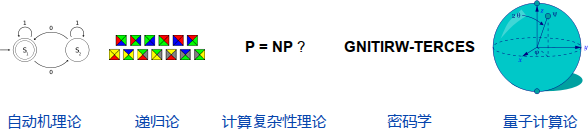
\includegraphics[scale=0.5]{theory_of_computation.png}
\caption{Theory of computation}
\label{theory_of_computation}
\end{figure}




\subsection{Information and coding theory}

Information theory is related to the quantification of information. This was developed by Claude E. Shannon to find fundamental limits on signal processing operations such as compressing data and on reliably storing and communicating data. Coding theory is the study of the properties of codes (systems for converting information from one form to another) and their fitness for a specific application. Codes are used for data compression, cryptography, error detection and correction, and more recently also for network coding. Codes are studied for the purpose of designing efficient and reliable data transmission methods.


信息论与信息量化相关,由Claude E. Shannon创建,用于寻找信号处理操作的根本极限,比如压缩数据和可靠的数据存储与通讯。编码理论是对编码以及它们适用的特定应用性质的研究。编码(code)被用于数据压缩,密码学,前向纠错,近期也被用于网络编码。研究编码的目的在于设计更高效、可靠的数据传输方法。




\subsection{Algorithms and data structures}

算法指定义良好的计算过程,它取一个或一组值作为输入,经过一系列定义好的计算过程,得到一个或一组输出。算法是计算机科学研究的一个重要领域,也是许多其他计算机科学技术的基础。算法主要包括数据结构、计算几何、图论等。除此之外,算法还包括许多杂项,如模式匹配、部分数论等。

\begin{figure}[!h]
\centering
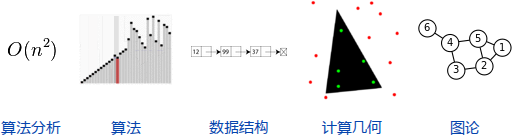
\includegraphics[scale=0.5]{algorithms.png}
\caption{Algorithms and data structure}
\label{algorithms_data_structure}
\end{figure}







\subsection{Programming language theory}

Programming language theory is a branch of computer science that deals with the design, implementation, analysis, characterization, and classification of programming languages and their individual features. It falls within the discipline of computer science, both depending on and affecting mathematics, software engineering and linguistics. It is an active research area, with numerous dedicated academic journals.

程序设计语言理论是计算机科学的一个分支,主要处理程序设计语言的设计、实现、分析、描述和分类,以及它们的个体特性。它属于计算机科学学科,既受影响于也影响着数学、软件工程和语言学。它是公认的计算机科学分支,同时也是活跃的研究领域,研究成果被发表在众多学术期刊,计算机科学以及工程出版物。

\begin{figure}[!h]
\centering
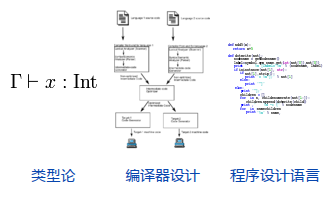
\includegraphics[scale=0.5]{programming_language.png}
\caption{Programming language}
\label{programming_language}
\end{figure}







\subsection{Formal methods}

Formal methods are a particular kind of mathematically based technique for the specification, development and verification of software and hardware systems. The use of formal methods for software and hardware design is motivated by the expectation that, as in other engineering disciplines, performing appropriate mathematical analysis can contribute to the reliability and robustness of a design. They form an important theoretical underpinning for software engineering, especially where safety or security is involved. Formal methods are a useful adjunct to software testing since they help avoid errors and can also give a framework for testing. For industrial use, tool support is required. However, the high cost of using formal methods means that they are usually only used in the development of high-integrity and life-critical systems, where safety or security is of utmost importance. Formal methods are best described as the application of a fairly broad variety of theoretical computer science fundamentals, in particular logic calculi, formal languages, automata theory, and program semantics, but also type systems and algebraic data types to problems in software and hardware specification and verification.

形式化方法是一种特别的基于数学的技术,用于软件和硬件系统的形式规范、开发以及形式验证。在软件和硬件设计方面,形式化方法的使用动机,如同其它工程学科,是通过适当的数学分析便有助于设计的可靠性和健壮性的期望。但是,使用形式化方法会带来很高的成本,意味着它们通常只用于高可靠性系统,这种系统中安全或保安(security)是最重要的。对于形式化方法的最佳形容是各种理论计算机科学基础种类的应用,特别是计算机逻辑演算,形式语言,自动机理论和形式语义学,此外还有类型系统、代数数据类型,以及软件和硬件规范和验证中的一些问题。








\section{Applied computer science}

Applied Computer Science aims at identifying certain Computer Science concepts that can be used directly in solving real world problems.



\subsection{Artificial intelligence}



This branch of computer science aims to or is required to synthesise goal-orientated processes such as problem-solving, decision-making, environmental adaptation, learning and communication which are found in humans and animals. From its origins in cybernetics and in the Dartmouth Conference (1956), artificial intelligence (AI) research has been necessarily cross-disciplinary, drawing on areas of expertise such as applied mathematics, symbolic logic, semiotics, electrical engineering, philosophy of mind, neurophysiology, and social intelligence. AI is associated in the popular mind with robotic development, but the main field of practical application has been as an embedded component in areas of software development which require computational understanding and modeling such as finance and economics, data mining and the physical sciences. The starting-point in the late 1940s was Alan Turing's question "Can computers think?", and the question remains effectively unanswered although the "Turing Test" is still used to assess computer output on the scale of human intelligence. But the automation of evaluative and predictive tasks has been increasingly successful as a substitute for human monitoring and intervention in domains of computer application involving complex real-world data.


这个计算机科学分支旨在创造可以解决计算问题,以及像动物和人类一样思考与交流的人造系统。无论是在理论还是应用上,都要求研究者在多个学科领域具备细致的、综合的专长,比如应用数学,逻辑,符号学,电机工程学,精神哲学,神经生理学和社会智力,用于推动智能研究领域,或者被应用到其它需要计算理解与建模的学科领域,如金融或是物理科学。人工智能领域开始变得正式源于Alan Turing这位人工智能先驱提出了图灵试验,以回答这样一个终极问题:“计算机能够思考吗?”

\begin{figure}[!h]
\centering
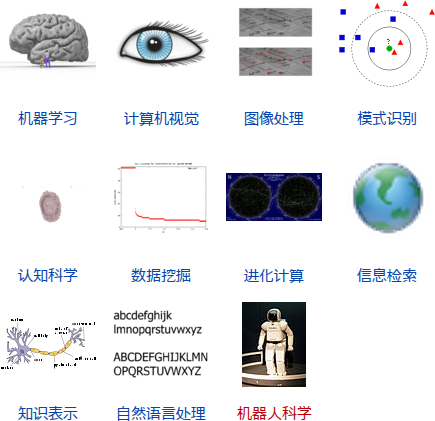
\includegraphics[scale=0.5]{ai.png}
\caption{人工智能}
\label{ai}
\end{figure}













\subsection{Computer architecture and engineering}




Computer architecture, or digital computer organization, is the conceptual design and fundamental operational structure of a computer system. It focuses largely on the way by which the central processing unit performs internally and accesses addresses in memory.[44] The field often involves disciplines of computer engineering and electrical engineering, selecting and interconnecting hardware components to create computers that meet functional, performance, and cost goals.

计算机系统结构,或者数字计算机组织,是一个计算机系统的概念设计和根本运作结构。它主要侧重于CPU的内部执行和内存访问地址。这个领域经常涉及计算机工程和电子工程学科,选择和互连硬件组件以创造满足功能、性能和成本目标的计算机。


\begin{figure}[!h]
\centering
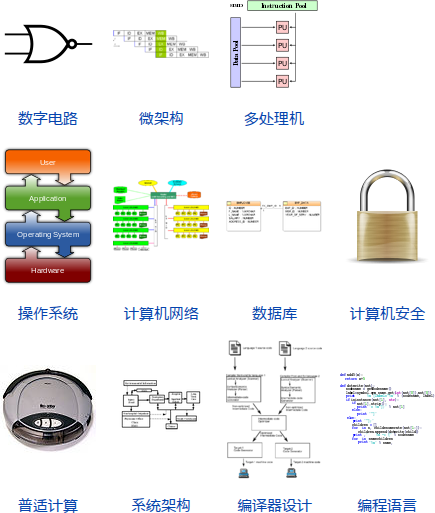
\includegraphics[scale=0.5]{computer_architecture.png}
\caption{Computer architecture}
\label{computer_architecture}
\end{figure}













\subsection{Computer graphics and visualization}



Computer graphics is the study of digital visual contents, and involves synthese and manipulations of image data. The study is connected to many other fields in computer science, including computer vision, image processing, and computational geometry, and is heavily applied in the fields of special effects and video games.

计算机图形学是对于数字视觉内容的研究,涉及图像数据的合成和操作。它跟计算机科学的许多其它领域密切相关,包括计算机视觉、图像处理和计算几何,同时也被大量运用在特效和电子游戏。






\subsection{Computer security and cryptography}



Computer security is a branch of computer technology, whose objective includes protection of information from unauthorized access, disruption, or modification while maintaining the accessibility and usability of the system for its intended users. Cryptography is the practice and study of hiding (encryption) and therefore deciphering (decryption) information. Modern cryptography is largely related to computer science, for many encryption and decryption algorithms are based on their computational complexity.

计算机安全是计算机技术的一个分支,其目标包括保护信息免受未经授权的访问、中断和修改,同时为系统的预期用户保持系统的可访问性和可用性。密码学是对于隐藏(加密)和破译(解密)信息的实践与研究。现代密码学主要跟计算机科学相关,很多加密和解密算法都是基于它们的计算复杂性。





\subsection{Computational science}


Computational science (or scientific computing) is the field of study concerned with constructing mathematical models and quantitative analysis techniques and using computers to analyze and solve scientific problems. In practical use, it is typically the application of computer simulation and other forms of computation to problems in various scientific disciplines.




\begin{figure}[!h]
\centering
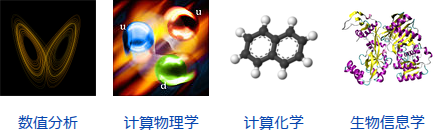
\includegraphics[scale=0.5]{scientific_computing.png}
\caption{科学计算}
\label{scientific_computing}
\end{figure}


计算科学(或者科学计算)是关注构建数学模型和量化分析技术的研究领域,同时通过计算机分析和解决科学问题。在实际使用中,它通常是计算机模拟和计算等形式在各个科学学科问题中的应用。





\subsection{Computer Networks}


This branch of computer science aims to manage networks between computers worldwide.







\subsection{Concurrent, parallel and distributed systems}

Concurrency is a property of systems in which several computations are executing simultaneously, and potentially interacting with each other. A number of mathematical models have been developed for general concurrent computation including Petri nets, process calculi and the Parallel Random Access Machine model. A distributed system extends the idea of concurrency onto multiple computers connected through a network. Computers within the same distributed system have their own private memory, and information is often exchanged amongst themselves to achieve a common goal.

并行性(concurrency)是系统的一种性质,这类系统可以同时执行多个可能互相交互的计算。一些数学模型,如Petri网、进程演算和PRAM模型,被创建以用于通用并发计算。分布式系统将并行性的思想扩展到了多台由网络连接的计算机。同一分布式系统中的计算机拥有自己的私有内存,它们之间经常交换信息以达到一个共同的目的。





\subsection{Databases and information retrieval}


A database is intended to organize, store, and retrieve large amounts of data easily. Digital databases are managed using database management systems to store, create, maintain, and search data, through database models and query languages.

数据库是为了更容易地组织、存储和检索大量数据。数据库由数据库管理系统管理,通过数据库模型和查询语言来存储、创建、维护和搜索数据。


\subsection{Health Informatics}

Health Informatics in computer science deals with computational techniques for solving problems in health care.




\subsection{Information science}


\begin{figure}[!h]
\centering

\includegraphics[scale=0.5]{information_science.png}
\caption{Information science}
\label{information_science}
\end{figure}



\subsection{Software engineering}

Software engineering is the study of designing, implementing, and modifying software in order to ensure it is of high quality, affordable, maintainable, and fast to build. It is a systematic approach to software design, involving the application of engineering practices to software. Software engineering deals with the organizing and analyzing of software— it doesn't just deal with the creation or manufacture of new software, but its internal maintenance and arrangement. Both computer applications software engineers and computer systems software engineers are projected to be among the fastest growing occupations from 2008 and 2018.

软件工程是对于设计、实现和修改软件的研究,以确保软件的高质量、适中的价格、可维护性,以及能够快速构建。它是一个系统的软件设计方法,涉及工程实践到软件的应用。


\chapter{The great insights of computer scicence}

According to many computer scientists, there are 3 Great Insights of Computer Science.

\begin{compactitem}
\item Bacon's, Leibniz's, Boole's, Alan Turing's, Shannon's, \& Morse's insight: There are only 2 objects that a computer has to deal with in order to represent "anything".

All the information about any computable problem can be represented using only 0 \& 1 (or any other bistable pair that can flip-flop between two easily distinguishable states,such as "on"/"off", "magnetized/de-magnetized", "high-voltage/low-voltage", etc.).


\item Alan Turing's insight: There are only 5 actions that a computer has to perform in order to do "anything".

Every algorithm can be expressed in a language for a computer consisting of only 5 basic instructions:

* move left one location

* move right one location

* print 0 at current-location

* print 1 at current-location

* erase current-location


\item Boehm and Jacopini's insight: There are only 3 ways of combining these actions (into more complex ones) that are needed in order for a computer to do "anything".

Only 3 rules are needed to combine any set of basic instructions into more complex ones:


\begin{compactitem}
\item sequence:

first do this; then do that

\item selection :

IF such-\&-such is the case,

THEN do this

ELSE do that

\item repetition:

WHILE such \& such is the case DO this


\end{compactitem}

Note that the 3 rules of Boehm's and Jacopini's insight can be further simplified with the use of goto (which means it's more elementary than structured programming.)

\end{compactitem}



\chapter{Academia}



\section{Conference}


Conferences are strategic events of the Academic Research in computer science. During those conferences, researchers from the public and private sectors present their recent work and meet. Proceedings of these conferences are an important part of the computer science literature.


\chapter{Education}


Some universities teach computer science as a theoretical study of computation and algorithmic reasoning. These programs often feature the theory of computation, analysis of algorithms, formal methods, concurrency theory, databases, computer graphics, and systems analysis, among others. They typically also teach computer programming, but treat it as a vessel for the support of other fields of computer science rather than a central focus of high-level study. The ACM/IEEE-CS Joint Curriculum Task Force "Computing Curriculum 2005" (and 2008 update)  gives a guideline for university curriculum.

Other colleges and universities, as well as secondary schools and vocational programs that teach computer science, emphasize the practice of advanced programming rather than the theory of algorithms and computation in their computer science curricula. Such curricula tend to focus on those skills that are important to workers entering the software industry. The process aspects of computer programming are often referred to as software engineering.

While computer science professions increasingly drive the U.S. economy, computer science education is absent in most American K-12 curricula. A report entitled "Running on Empty: The Failure to Teach K-12 Computer Science in the Digital Age" was released in October 2010 by Association for Computing Machinery (ACM) and Computer Science Teachers Association (CSTA), and revealed that only 14 states have adopted significant education standards for high school computer science. The report also found that only nine states count high school computer science courses as a core academic subject in their graduation requirements. In tandem with "Running on Empty", a new non-partisan advocacy coalition - Computing in the Core (CinC) - was founded to influence federal and state policy, such as the Computer Science Education Act, which calls for grants to states to develop plans for improving computer science education and supporting computer science teachers.

Within the United States a gender gap in computer science education has been observed as well. Research conducted by the WGBH Educational Foundation and the Association for Computing Machinery (ACM) revealed that more than twice as many high school boys considered computer science to be a “very good” or “good” college major than high school girls. In addition, the high school Advanced Placement (AP) exam for computer science has displayed a disparity in gender. Compared to other AP subjects it has the lowest number of female participants, with a composition of about 15 percent women. This gender gap in computer science is further witnessed at the college level, where 31 percent of undergraduate computer science degrees are earned by women and only 8 percent of computer science faculty consists of women. According to an article published by the Epistemic Games Group in August 2012, the number of women graduates in the computer science field has declined to 13 percent


一些教授计算机科学的大学主要进行计算和算法推理的研究。其中包括计算理论、算法分析、形式化方法、并行理论、数据库、计算机图形学以及系统分析等。通常也教授程序设计,但仅仅将它看作是支持计算机科学其它领域的媒介,而不是高级研究的重心。


其它一些学院、大学、中学以及职业培训的计算机科学课程则主要侧重于训练高级编程,而不是算法和计算理论。这些课程着重教授那些对于软件工业很重要的技能。像这样的计算机编程过程通常被叫做软件工程。

然而,尽管计算机科学专业日益推动着美国经济,但是计算机科学教育依然不存在大多数美国K-12课程中。2010年10月由ACM和计算机科学教师协会(CSTA)共同发表了一篇名为“Running on Empty: The Failure to Teach K-12 Computer Science in the Digital Age”的报告,文中揭示了仅有14个州通过了有意义的高中计算机科学教育标准。同时,仅有9个州将高中计算机科学课程算作毕业要求的核心学科。配合“Running on Empty”这篇文章,一个新的无党派宣传联盟:Computing in the Core(CinC)被创建,以影响联邦和政府政策,比如Computer Science Education Act要求政府拨款以制定计划完善计算机科学教育及支持计算机科学教师。



